\documentclass{DateStructure}

\SubjectName{家庭族谱的构建}
\CollegeName{理学院}
\Major{信息与计算科学}
\GroupNumber{第十六组}
\StudentA{20071226}{童繁}{流程图}
\StudentB{20071227}{王瀚功}{测试}
\StudentC{20071228}{王赛豪}{文案}
\StudentD{20071229}{吴政豪}{调试}
\StudentE{20071230}{武琦}{代码}

\begin{document}
\makecover
\newpage
\thispagestyle{empty}
\tableofcontents   
\newpage
\setcounter{page}{1}  

\section{需求分析}
\begin{itemize}
\item[(1)]利用二叉树的存储结构,使用孩子兄弟表示法,将本人的家谱进行存储、查询和显示等功能。
\item[(2)]输入:根据姓名和其父名字,插入族谱中相应的位置。
\item[(3)]查询:根据输入的姓名,查找其在该族谱中属于第几代。
\item[(3)]输出:以可视化的方式对族谱进行输出。
\end{itemize}

\section{项目亮点}
\begin{itemize}
\item[(1)]建立了家谱的初始化和保存机制;
\item[(2)]利用了二叉树的存储结构,使用孩子兄弟表示法完成了家谱管理系统;
\item[(3)]以凹入表的形式打印家谱;
\item[(4)]设计了成员信息合法的检查函数;
\item[(5)]添加了删除成员的功能;
\item[(6)]添加了修改成员信息的功能。
\end{itemize}

\section{概要设计}
族谱记录的是同姓的亲人,一般是男性及其后代。对于出嫁的女性,若其后代随父姓,则不记录在本族家谱内;若随母姓,则记录在本族家谱内。\par
家谱中成员的信息包括:姓名、性别、配偶姓名、辈分、出生日期、是否在世、父亲或母亲的姓名(本家姓)。在修改成员信息的功能中有“记录过世”这一选项,如果家谱中某位成员刚刚过世,在记录时会弹出:“逝者安息,生者奋然。”\par
程序运行时,首先初始化,读取家谱文件生成一个孩子兄弟树,用户选择功能执行。用户选择退出时,将更新的家谱保存到文件后结束程序。\par
\begin{figure}[H] 
\centering
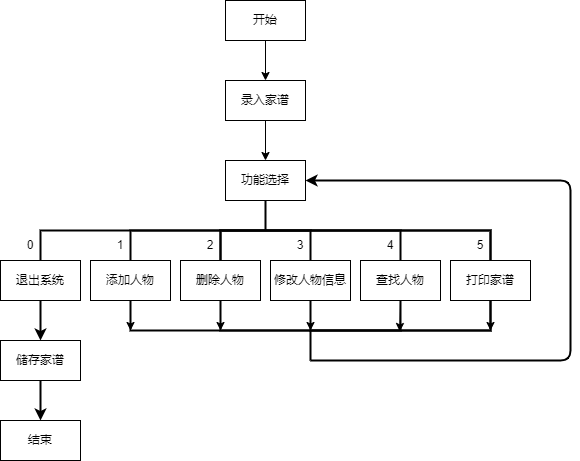
\includegraphics[width=\linewidth]{main.png}
\caption{主函数流程图}
\end{figure}

\section{详细设计}
\subsection{定义}
\begin{figure}[H] 
\centering
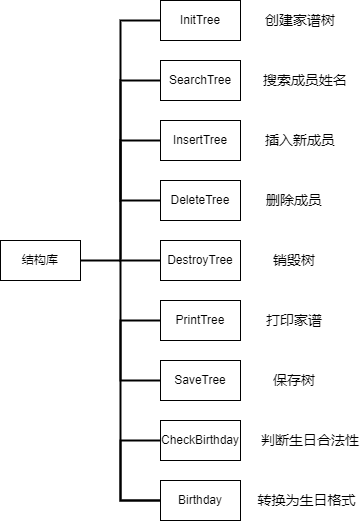
\includegraphics[width=300pt]{tree.png}
\caption{结构函数库}
\end{figure}
\begin{figure}[H] 
\centering
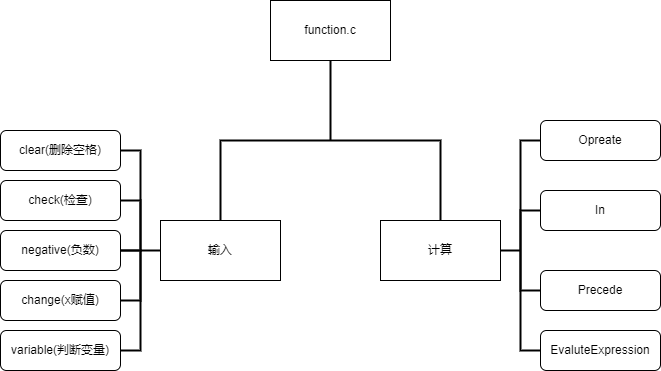
\includegraphics[width=300pt]{function.png}
\caption{功能函数库}
\end{figure}
\lstinputlisting[language=C]{./code/definition.h}	
\subsection{重要函数}
\subsubsection{添加成员}
\begin{figure}[H] 
\centering
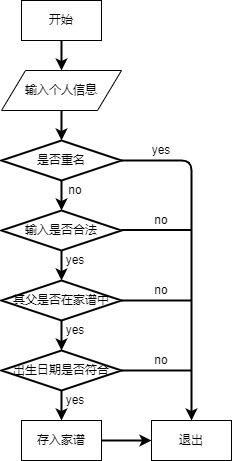
\includegraphics[width=250pt]{insert.png}
\caption{添加成员}
\end{figure}
\begin{lstlisting}[language=c,caption={Insert}]
Status Insert()//添加成员
{
    char father[20];
    A=NULL;B=NULL;
    InitTree(&A);
    printf("请输入:姓名(不能重名) 性别(男1|女0) 配偶姓名(没有输入无) 出生日期(8位数) 是否在世(1|0) 父亲姓名\n ");
    scanf("%s %d %s %d %d %s",&A->data.name,&A->data.sex,&A->data.spouse,&A->data.birthday,&A->data.alive,father);
    SearchTree(T,A->data.name,&B);
    if(B!=NULL)
    {
        printf("姓名与家族成员重名!\n");
        free(A);
        A=NULL;
        return ERROR;
    }
    B=NULL;
    if(A->data.sex!=1&&A->data.sex!=0)
    {
        printf("性别输入有误!\n");
        free(A);
        A=NULL;
        return ERROR;
    }
    if(A->data.alive!=1&&A->data.alive!=0)
    {
        printf("莫把生命当儿戏!\n");
        free(A);
        A=NULL;
        return ERROR;
    }
    if(!CheckBirthday(A->data.birthday))
    {
        printf("出生日期输入有误!\n");
        free(A);
        A=NULL;
        return ERROR;
    }
    SearchTree(T,father,&B);
    if(B==NULL)
    {
        printf("此人的父亲不在家谱里!\n");
        free(A);
        A=NULL;
        return ERROR;
    }
    if(B->data.seniority!=0&&B->data.birthday>=A->data.birthday)
    {
        printf("出生日期不能比父亲早!\n");
        free(A);
        A=NULL;
        B=NULL;
        return ERROR;
    }
    InsertTree(&B,&A);
    printf("添加了新的家庭成员!\n");
    A=NULL;
    return OK;
}
\end{lstlisting}
\subsubsection{删除成员}
\begin{figure}[H] 
\centering
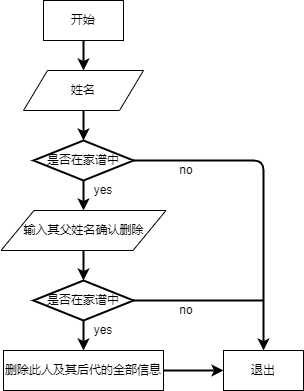
\includegraphics[width=300pt]{delete.png}
\caption{删除成员}
\end{figure}
\begin{lstlisting}[language=c,caption={Delete}]
Status Delete()//删除成员
{
    A=NULL;B=NULL;
    char name[20],fatherName[20];
    printf("请输入姓名:");
    scanf("%s",name);
    SearchTree(T,name,&A);
    if(A==NULL)
    {
        printf("不存在名为%s的人\n",name);
        return ERROR;
    }
    printf("请输入其父亲的名字确定删除:");
    scanf("%s",fatherName);
    SearchTree(T,fatherName,&B);
    if(B==NULL)
    {
        printf("此人的父亲不在家谱里!\n");
        return ERROR;
    }
    DeleteTree(&A);
    printf("已删除%s及其后代的全部信息!\n",name);
    A=NULL;B=NULL;
    return OK;
}
\end{lstlisting}
\subsubsection{修改成员信息}
\begin{figure}[H] 
\centering
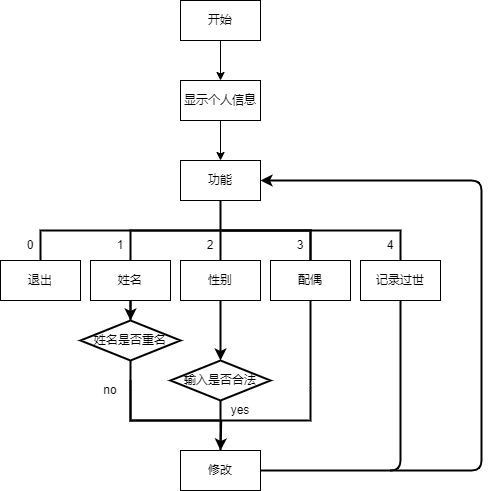
\includegraphics[width=300pt]{edit.png}
\caption{修改成员信息}
\end{figure}
\begin{lstlisting}[language=c,caption={Edit}]
Status Edit(Tree *B,Forest T)//修改成员信息
{
    if((*B)==NULL) return ERROR;
    if((*B)->data.seniority==0)
    {
        printf("该节点为森林根结点,禁止操作!\n");
        system("pause");
        return ERROR;
    }
    int choice; 
    A:system("cls");
    Show(&(*B));
    printf("\n您想修改什么信息?\n\n");
    printf("********************************\n");
    printf("0.退出   1.姓名   2.性别   3.配偶   4.记录过世(慎重选择)\n");
    printf("********************************\n");		        
	printf("请输入序号:");
    fflush(stdin);
    scanf("%d",&choice);
    switch(choice)
    {
        case 1:
            printf("请输入新名字:");
            char name[20];
            fflush(stdin);
            scanf("%s",name);
            Tree D;
            SearchTree(T,name,&D);
            if(D!=NULL) printf("与其他家庭成员重名!\n");
            else strcpy((*B)->data.name,name);
            system("pause");goto A;
        case 2:
            printf("你的性别为(男1|女0):");
            int sex;
            fflush(stdin);
            scanf("%d",&sex);
            if(sex!=0&&sex!=1)
            {
                printf("输入有误\n");
                system("pause"); goto A;
            }
            (*B)->data.sex=sex;
            system("pause"); goto A;
        case 3:
            printf("请输入配偶姓名:");
            char spouse[100];
            fflush(stdin);
            scanf("%s",spouse);
            strcpy((*B)->data.spouse,spouse);
            system("pause"); goto A;
		case 4:
            if((*B)->data.alive) (*B)->data.alive=0;
            printf("逝者安息,生者奋然。\n");
            system("pause"); goto A;
        case 0:break;
        default:goto A;
    } 
    return OK; 
}
\end{lstlisting}

\section{用户手册}
\subsection{界面}
\begin{figure}[H] 
\centering
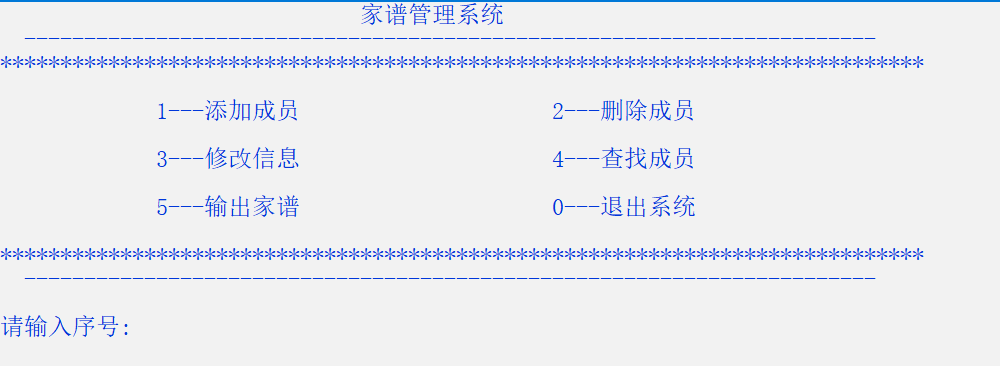
\includegraphics[width=300pt]{界面.png}
\caption{界面}
\end{figure}
\subsection{删除成员}
\begin{figure}[H] 
\centering
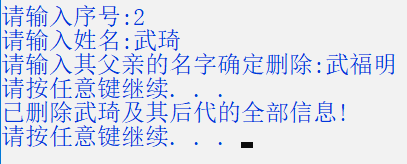
\includegraphics[width=300pt]{删除成员.png}
\caption{删除成员}
\end{figure}
\subsection{添加成员}
\begin{figure}[H] 
\centering
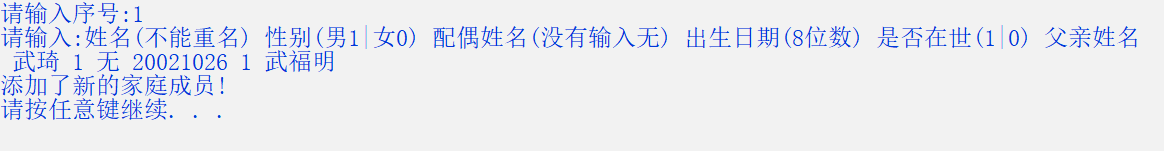
\includegraphics[width=\linewidth]{添加成员.png}
\caption{添加成员}
\end{figure}
\subsection{查找成员}
\begin{figure}[H] 
\centering
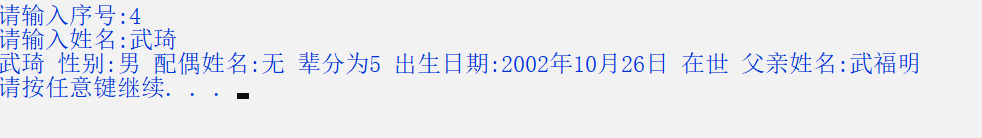
\includegraphics[width=\linewidth]{查找成员.png}
\caption{查找成员}
\end{figure}
\subsection{修改成员信息}
\begin{figure}[H] 
\centering
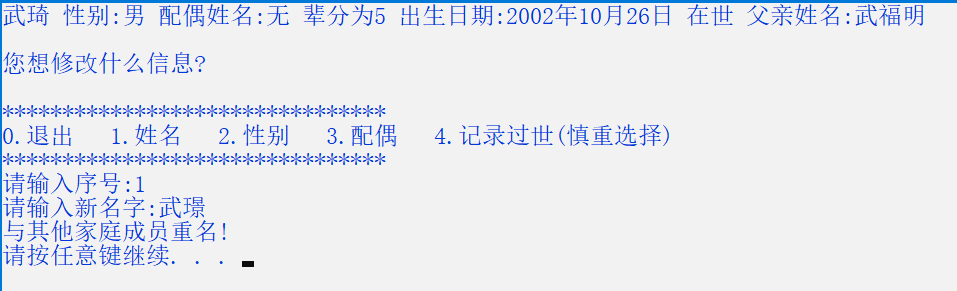
\includegraphics[width=\linewidth]{修改成员信息.png}
\caption{修改成员信息}
\end{figure}


\section{心得体会}
这次课程设计的心得体会通过实践我们的收获如下:\par
1.在这次的家庭族谱构建过程中,我们更深刻地了解了二叉树的特点与用法。\par
2.在做一个较大的程序过程中,应该学会边编写程序边运行,即完成了一个功能,也要对其调试,这样有利于我们高效地完成项目,并在调试BUG的过程可以大大减小难度。\par
3.必须要有良好的编程习惯。首先编码风格要统一规范,这样不仅有利于代码的阅读,更有利于代码的维护。其次在一些代码方面要细心谨慎,减少BUG出现的机率。\par
4.更加系统地学习了C语言的system函数,对goto函数的运用更加熟练。\par

\newpage 
\section{附录}
\subsection{definition.h}
\lstinputlisting[language=C]{./code/definition.h}
\subsection{main.c}
\lstinputlisting[language=C]{./code/main.c}
\subsection{tree.c}
\lstinputlisting[language=C]{./code/tree.c}
\subsection{function.c}
\lstinputlisting[language=C]{./code/function.c}

\end{document}
